\begin{figure}[htbp]
    \centering
    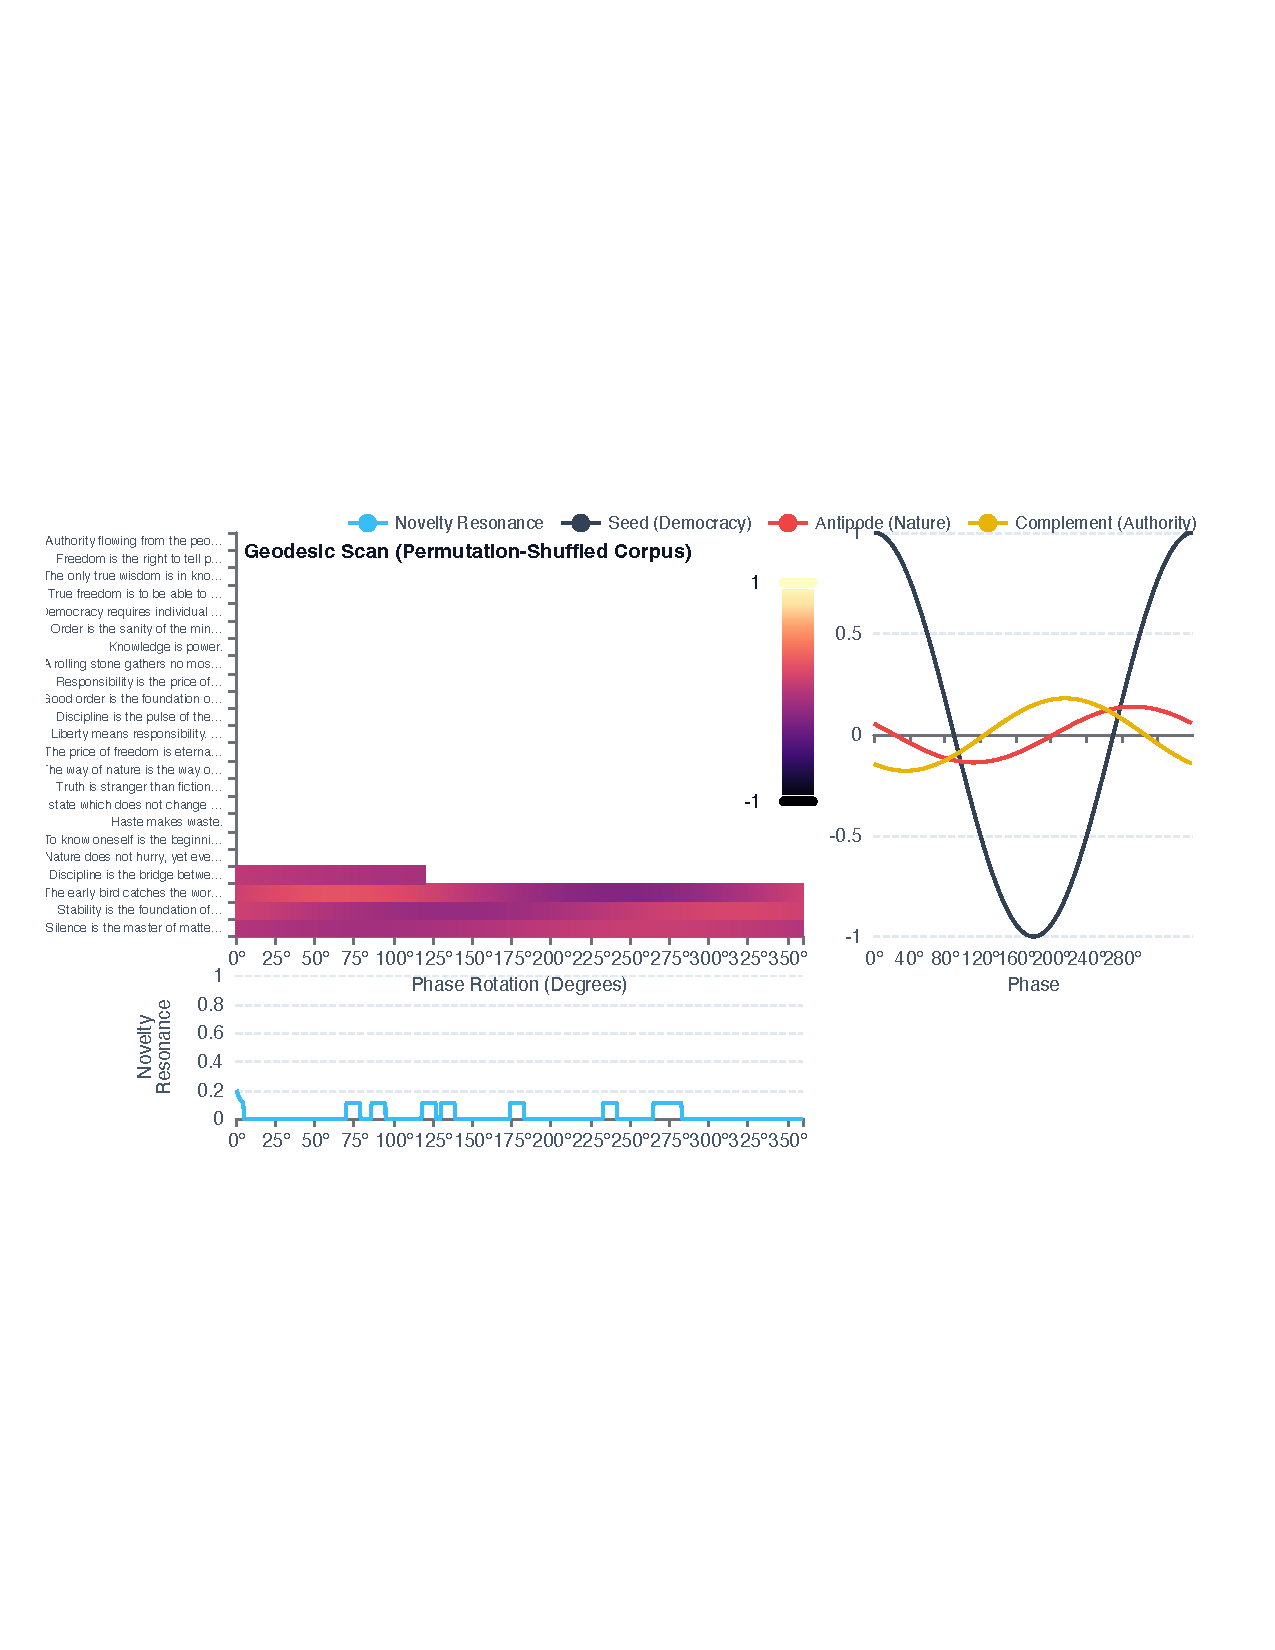
\includegraphics[width=1.0\textwidth]{ permutation_metrics_chart.pdf }
    \caption{ (Left, Top) Semantic geodesic matrix mapping geometric score across corpus as query phase rotates 360°. (Left, Bottom) Novelty resonance showing where top match changes. (Right) Spectral complementarity: cosine similarity of the rotating seed to named items, showing pure U(1) sinusoidal structure. }
    \label{ fig:permutation_metrics }
\end{figure}
